% !TeX spellcheck = en_US
\documentclass[10pt]{beamer}
\usepackage[latin1]{inputenc}
\usetheme{Warsaw}
\usecolortheme{beaver}
%\usepackage{braket}
\usepackage{amsmath}
\usepackage{amsfonts}
\usepackage{amssymb}
\usepackage{graphicx}
%\setbeamerfont{page number in head/foot}{size=\normalsize}
%\setbeamertemplate{footline}[frame number]

\newcommand*\oldmacro{}%
\let\oldmacro\insertshorttitle%
\renewcommand*\insertshorttitle{%
	\oldmacro\hfill%
	\insertframenumber\,/\,\inserttotalframenumber}
\setbeamercovered{transparent}
\usepackage{tikz}
\usetikzlibrary{calc}
\usepackage{pgfplots}
\usepackage{tikz-3dplot}
\usetikzlibrary{decorations.markings}
\usetikzlibrary{shapes,arrows}
\newcommand{\midarrowright}{\tikz \draw[-triangle 90] (0,0) -- +(.1,0);}
\newcommand{\midarrowup}{\tikz \draw[-triangle 90] (0,0) -- +(0,.1);}

\usetikzlibrary{shadings, calc, decorations.markings}
\tikzset{->-/.style={decoration={
			markings,
			mark=at position #1 with {\arrow{>}}},postaction={decorate}},
	->-/.default=0.5,
}


\newcommand\ds{\displaystyle}
\newcommand\ts{\textstyle}
\newcommand{\mb}{\mathbf}
%\renewcommand{\thenotation}{}
%\renewcommand{\theequation}{\thesection.\arabic{equation}}
\def\Caption #1{\caption{\footnotesize #1}}
%\renewcommand\Caption{#1}{\Caption{\small{#1}}}
%\def\Caption #1{\Caption{\small{{#1}}}}

\def \Bfemph #1{\textbf{\emph{#1}}}


%\def\Proof.{{\medbreak\noindent{\it Dimostrazione}\enspace}}
\def\Proof{{\medbreak\noindent{\textbf{Proof.} }}}
\def\Proofsketch{{\medbreak\noindent{\textbf{Sketch of proof.} }}}
\def\endproof{~\hfill $\blacksquare$}
%\def\endproof{\hfill$\square$\par\medskip}

\def\Svolgimento{{\medbreak\noindent{\textit{Execution.} }}}
\def\Suggerimento{{\medbreak\noindent{\textit{Hint:} }}}


\def\mR{{\mathbb R}}
\def\mC{{\mathbb C}}
\newcommand{\parz}[2]{ \frac{\partial #1}{\partial #2}}
\newcommand{\deri}[2]{\displaystyle \frac{\dd #1}{\dd #2}}
\renewcommand{\Re}{\text{Re }}
\renewcommand{\Im}{\text{Im }}
%\renewcommand{\theta}{\vartheta}
\newcommand{\Int}{\text{Int }}
\newcommand{\Ext}{\text{Ext }}
\newcommand{\supp}{\text{supp}}
\newcommand{\mD}{\mathcal{D}}
\newcommand{\dd}{\mathrm d}
\newcommand{\norm}[1]{\displaystyle \left \| #1 \right \|}
\renewcommand{\div}{\operatorname{div}}
\newcommand{\rot}{\operatorname{rot}}
\newcommand{\grad}{\operatorname{grad}}
\newcommand{\id}{\mathds{1}}
\newcommand{\mM}{\mathrm{M}}
\newcommand{\mT}{\mathrm{T}}
%\renewcommand{\to}{\longrightarrow}
\newcommand{\scalar}[2]{\left\langle #1, #2 \right\rangle}
\newcommand{\mf}[1]{\mathbf{#1}}

\def\Xint#1{\mathchoice 
	{\XXint\displaystyle\textstyle{#1}}% 
	{\XXint\textstyle\scriptstyle{#1}}% 
	{\XXint\scriptstyle\scriptscriptstyle{#1}}% 
	{\XXint\scriptscriptstyle\scriptscriptstyle{#1}}% 
	\!\int} 
\def\XXint#1#2#3{{\setbox0=\hbox{$#1{#2#3}{\int}$} 
		\vcenter{\hbox{$#2#3$}}\kern-.5\wd0}} 
\def\Mint{\Xint -}


\renewcommand{\hat}[1]{\widehat{#1}}
\renewcommand{\theta}{\vartheta}
\renewcommand{\epsilon}{\varepsilon}
%\renewcommand{\phi}{\varphi}
\newcommand{\res}{\mathop{\mathrm{Res }}}

\newcommand{\colonna}[2]{\begin{pmatrix}
		#1 \\ #2
\end{pmatrix}}
\newcommand{\riga}[2]{\begin{pmatrix}
		#1 & #2
\end{pmatrix}}
%%%%%%%%%%%%%%%%%%%%%%%%%%%%%%%%%%%%%%%%%%%%%%%%%%%%%%%%%%%%%%%%%%%%%%%%%%%%%%%%%%%%%%%%%%%



\title{Soluzioni fondamentali per equazioni di tipo onda su variet� curve}
\author{Rubens Longhi}
\date


\begin{document}
	
	
	\begin{frame}
	 \maketitle
	 	\begin{center}
	 	\[\Box u=\delta\]
	 	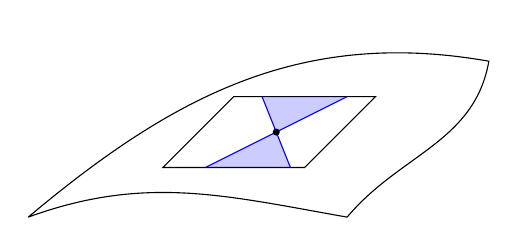
\begin{tikzpicture}[scale=0.9]
	 	\tikzstyle{every node}=[font=\scriptsize]
	 	
	 	\draw (1,2.8) to[out=40,in=170] (7.5,5) %node at (7,4.8) {$\mathrm{M}$}
	 	to[out=-100,in=50]  (5.5,2.8) to[out=170,in=20] (1,2.8);
	 	
	 	\begin{scope}[shift={(0.5,0)},scale=1]
	 	\clip (2.2,3.4)-- (4.7,3.4) -- (5.7,4.6) -- (3.2,4.6) -- cycle;
	 	\draw [draw=black, thin, fill=white] (2.4,3.5)-- (4.4,3.5) -- (5.4,4.5) -- (3.4,4.5) -- cycle;
	 	%\draw [ultra thin, dashed] (1,2.8) to[out=40,in=170] (7.5,5) %node at (7,4.8) {$\mathrm{M}$}
	 	% to[out=-100,in=50]  (5.5,2.8) to[out=170,in=20] (1,2.8);
	 	
	 	\draw [thin, color=blue, fill=blue, fill opacity=0.2] (3,3.5) -- (4,4) -- (4.2,3.5) ;
	 	
	 	\draw [thin, color=blue, fill=blue, fill opacity=0.2] (3.8,4.5) -- (4,4) -- (5,4.5);
	 	
	 	%\draw [thin, color=blue, fill=blue, fill opacity=0.2] (3,3.5) -- (5,4.5)-- (3.8,4.5) -- (4.2,3.5) -- (3.8,4.5);
	 	\fill [black] (4,4) circle (0.05cm) %node [left] {$x$}
	 	;
	 	\end{scope}
	 	
	 	%\node at (5.3,4) {$\mathrm{T}_x\mathrm{M}$};
	 	
	 	\end{tikzpicture}
	\end{center}
	\begin{center}
		
	\end{center}

	\end{frame}
	
	\begin{frame}
		\frametitle{Equazioni di tipo ondulatorio}
		\framesubtitle{Un preambolo}
\tikzstyle{na} = [baseline=-.5ex]

Gli operatori di tipo ondulatorio $P$ appaiono in molti sistemi fisici
\begin{itemize}[<+-| alert@+>]
	\item Operatore d'onda: il d'Alembertiano\\

	$$\displaystyle \Box=\frac{\partial^2}{\partial t^2}-\sum_{j=1}^{n-1}\frac{\partial^2}{\partial x_j^2}$$
	
	%\tikz[na] \node[coordinate] (n1) {};
\end{itemize}

% Below we mix an ordinary equation with TikZ nodes. Note that we have to
% adjust the baseline of the nodes to get proper alignment with the rest of
% the equation.
\begin{itemize}[<+-| alert@+>]
	\item Equazioni di Maxwell
\begin{equation*}
\Box A^\mu-\partial^\mu\partial_\nu A^\nu=4\pi J^\mu
\end{equation*}
\end{itemize}

\begin{itemize}[<+-| alert@+>]
	\item Equazione di Klein-Gordon
	\begin{equation*}
	(\Box +m^2)\psi=0
	\end{equation*}
\end{itemize}




\end{frame}


\begin{frame}
	\frametitle{Le soluzioni fondamentali}
	\framesubtitle{Un metodo costruttivo}
	
	Vogliamo risolvere su una variet� $\mM$ una qualsiasi equazione differenziale non omogenea \[	Pf=\psi		\] nell'incognita $f$ con generica sorgente $\psi$.\\ \pause
	\bigskip
	La studiamo nel caso di una sorgente elementare deltiforme nel punto $x$ \[	Pu_x=\delta_x		\]
	e cerchiamo soluzioni distribuzionali $u_x\in\mD'(\mM)$.\\	\pause
	\bigskip		
	Troviamo una soluzione a $Pf=\psi$ integrando opportunamente la soluzione fondamentale su tutti i punti $x\in\supp\,\psi$.

	
	
	
	
	
\end{frame}


\begin{frame}
	
	\frametitle{L'operatore d'onda in Minkowski}
	\framesubtitle{Il caso dello spaziotempo piatto}
	
	La simmetria per traslazione ci consente di limitare il problema per $\Box$ all'origine: $$ \Box u_0=\delta_0$$ e di utilizzare la tecnica della trasformata di Fourier.\\ \pause
	\bigskip
	La PDE in $(t,\mf{x})$ diventa l'equazione algebrica nello spazio delle fasi $(\omega,\mf{k})$
	\[	(|\mf{k}|^2-\omega^2)\widehat{u}=1,	\]
	della quale troviamo \textcolor{red}{\textbf{due soluzioni indipendenti}}, che danno luogo a due soluzioni fondamentali $G^+$ e $G^-$ dette \textcolor{red}{\textbf{ritardata}} e \textcolor{red}{\textbf{avanzata}}.
	
	
	
	
\end{frame}




\begin{frame}
	\framesubtitle{Le soluzioni fondamentali in Minkowski}
	\frametitle{Il caso $n=1+1$ - onde su una corda}
 		
	 
	\begin{columns}[t]
		\begin{column}{.48\linewidth}
		
			\begin{block}
				
				\begin{figure}
					\centering
					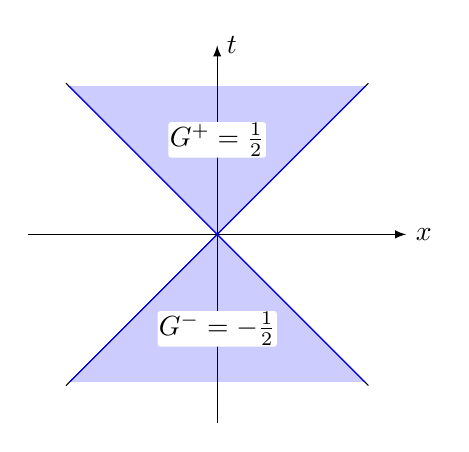
\begin{tikzpicture}[scale=0.48][>=latex]
						\coordinate (Origin)   at (0,0);
					\coordinate (XAxisMin) at (-5,0);
					\coordinate (XAxisMax) at (5,0);
					\coordinate (YAxisMin) at (0,-5);
					\coordinate (YAxisMax) at (0,5);
					\draw [thin,-latex] (XAxisMin) -- (XAxisMax) node[right] {$x$};% Draw x axis
					\draw [thin,-latex] (YAxisMin) -- (YAxisMax) node[right] {$t$};% Draw y axis
					
					%\clip (-5,-5) rectangle (10cm,10cm); % Clips the picture...
					
					\onslide<1>{\draw[thin] (0,0) -- (4,4);
						\draw[thin] (0,0) -- (-4,4);
						\begin{scope}
						\clip (-4,0) -- (4,0) -- (4,3.9)-- (-4,3.9) --cycle;
						\draw [thin, color=blue, fill=blue, fill opacity=0.2] (0,0) -- (4,4) -- (-4,4) --cycle ;
						\end{scope}
						\node[fill=white,rounded corners=1pt,inner sep=0.5pt] at (0,2.5) {$G^+=\frac{1}{2}$};
						
					}
				
					\onslide<2>{\draw[thin] (0,0) -- (4,-4);
						\draw[thin] (0,0) -- (-4,-4);
						\begin{scope}
						\clip (-4,0) -- (4,0) -- (4,-3.9)-- (-4,-3.9) --cycle;
						\draw [thin, color=blue, fill=blue, fill opacity=0.2] (0,0) -- (4,-4) -- (-4,-4) --cycle ;
						\end{scope}
						\node[fill=white,rounded corners=1pt,inner sep=0.5pt] at (0,-2.5) {$G^-=-\frac{1}{2}$};
					}
					
					
					
					
					
					
					\end{tikzpicture}
				\end{figure}
			\end{block}
			
		\end{column}
		
		\begin{column}{.48\linewidth}
			
			\only<1>{La soluzione fondamentale \textcolor{red}{\textbf{ritardata}} \[	G^{+}(t,x)=\frac{\Theta(t-|x|)}{2}	\]
				$\supp\, G^+$ � il cono luce \textcolor{red}{\textbf{futuro}}
					}
			\only<2>{La soluzione fondamentale \textcolor{red}{\textbf{avanzata}} \[	G^{-}(t,x)=-\frac{\Theta(t+|x|)}{2}	\]	$\supp\, G^-$ � il cono luce \textcolor{red}{\textbf{passato}}}
			
			
			
		\end{column}
		
		
		
		
	\end{columns}
	
	
	
	
	
	
\end{frame}




\begin{frame}
	\framesubtitle{Le soluzioni fondamentali in Minkowski}
	\frametitle{Il caso $n=1+2$ - onde su una superficie}
	
	\begin{columns}[t]
		\begin{column}{.48\linewidth}
			
			\begin{block}
				
				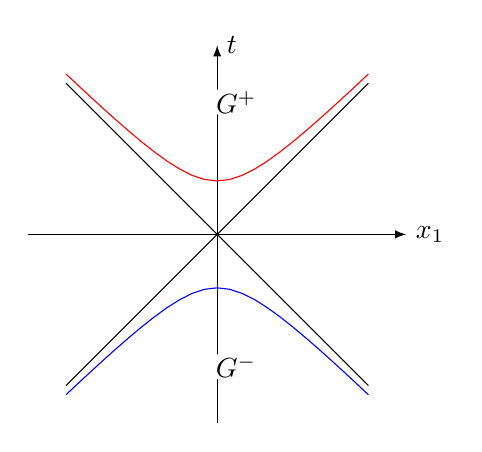
\begin{tikzpicture}[scale=0.48][>=latex]
				\coordinate (Origin)   at (0,0);
				\coordinate (XAxisMin) at (-5,0);
				\coordinate (XAxisMax) at (5,0);
				\coordinate (YAxisMin) at (0,-5);
				\coordinate (YAxisMax) at (0,5);
				\draw [thin,-latex] (XAxisMin) -- (XAxisMax) node[right] {$x_1$};% Draw x axis
				\draw [thin,-latex] (YAxisMin) -- (YAxisMax) node[right] {$t$};% Draw y axis
				%\draw [thin,-latex] (1.5,0.75) -- (-3,-1.5) node[left] {$x_2$};% Draw x axis
				
				%\clip (-5,-5) rectangle (10cm,10cm); % Clips the picture...
				
				\draw[thin] (0,0) -- (4,4);
				\draw[thin] (0,0) -- (-4,4);
				
				\onslide<1>{	\draw[red] plot[domain=-4:4] (\x,{sqrt(\x* \x+2)});
					\node[fill=white,rounded corners=1pt,inner sep=0.5pt] at (0.5,3.5) {$G^+$};}
			
				
				\draw[thin] (0,0) -- (4,-4);
				\draw[thin] (0,0) -- (-4,-4);
				\onslide<2>{\draw[blue] plot[domain=-4:4] (\x,{-sqrt(\x* \x+2)});
					\node[fill=white,rounded corners=1pt,inner sep=0.5pt] at (0.5,-3.5) {$G^-$};}
				
				
				
				
				
				
				
				\end{tikzpicture}
			\end{block}
			
		\end{column}
	
	\begin{column}{.48\linewidth}
		
		\only<1>{Un insieme di livello della soluzione fondamentale \textcolor{red}{\textbf{ritardata}} \[	G^{+}(t,\mf{x})=\frac{\Theta( t)}{2\pi}\frac{\Theta(t^2-|\mf{x}|^2)}{\sqrt{t^2-|\mf{x}|^2}}	\]
		$\supp\, G^+\subset$ cono luce \textcolor{red}{\textbf{futuro}}}
		\only<2>{Un insieme di livello della soluzione fondamentale \textcolor{red}{\textbf{avanzata}} \[	G^{-}(t,\mf{x})=\frac{\Theta(-t)}{2\pi}\frac{\Theta(t^2-|\mf{x}|^2)}{\sqrt{t^2-|\mf{x}|^2}}	\]	$\supp\, G^-\subset$ cono luce \textcolor{red}{\textbf{passato}}}
	\end{column}
	
	\end{columns}
	
	
	
	
	
	
\end{frame}

\begin{frame}
	\framesubtitle{Le soluzioni fondamentali in Minkowski}
	\frametitle{Il caso $n=1+3$ - onde nello spazio}
	
	\begin{columns}[t]
		\begin{column}{.48\linewidth}
			
			\begin{block}
				
			\only<1>{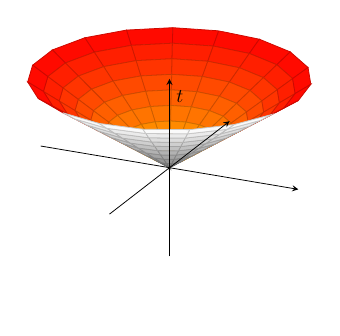
\begin{tikzpicture}[scale=0.7]
			\pgfplotsset{ticks=none}
			\begin{axis}[
			axis lines=center,
			axis on top,
			xlabel={}, ylabel={}, zlabel={$t$},
			domain=0:1,
			y domain=0:2*pi,
			%domain=-1:1,
			%y domain=-1:1,
			xmin=-1.5, xmax=1.5,
			ymin=-1.5, ymax=1.5, zmin=-1.0,
			%every axis x label/.style={at={(rel axis cs:0,0.5,0)},anchor=south},
			%every axis y label/.style={at={(rel axis cs:0.5,0,0)},anchor=north},
			every axis z label/.style={at={(rel axis cs:0.5,0.5,0.9)},anchor=west},
			mesh/interior colormap name=hot,
			colormap/blackwhite, 
			%samples=40,
			%samples y=60,
			samples=10,
			samples y=20,
			z buffer=sort,
			]
			\addplot3 [ surf, shader=faceted] ({(1.5*x*cos(deg(y))},{1.5*x*sin(deg(y))},{x});
			\addplot3 [opacity=0, fill opacity=0, surf, shader=faceted] ({(1.5*(-x)*cos(deg(y))},{1.5*(-x)*sin(deg(y))},{-x});
			
			
			\end{axis}
			\end{tikzpicture}}
	
		
		\only<2>{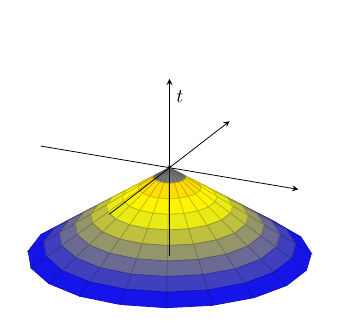
\begin{tikzpicture}[scale=0.7]
		\pgfplotsset{ticks=none}
		\begin{axis}[
		axis lines=center,
		axis on top,
		xlabel={}, ylabel={}, zlabel={$t$},
		domain=0:1,
		y domain=0:2*pi,
		%domain=-1:1,
		%y domain=-1:1,
		xmin=-1.5, xmax=1.5,
		ymin=-1.5, ymax=1.5, zmin=-1.0,
		%every axis x label/.style={at={(rel axis cs:0,0.5,0)},anchor=south},
		%every axis y label/.style={at={(rel axis cs:0.5,0,0)},anchor=north},
		every axis z label/.style={at={(rel axis cs:0.5,0.5,0.9)},anchor=west},
		mesh/interior colormap name=hot,
		colormap/blackwhite, 
		%samples=40,
		%samples y=60,
		samples=10,
		samples y=20,
		z buffer=sort,
		]
		\addplot3 [opacity=0, fill opacity=0, surf, shader=faceted] ({(1.5*x*cos(deg(y))},{1.5*x*sin(deg(y))},{x});
		\addplot3 [surf, shader=faceted] ({(1.5*(-x)*cos(deg(y))},{1.5*(-x)*sin(deg(y))},{-x});
			
			
			\end{axis}
			\end{tikzpicture}}
		
			\end{block}
			
		\end{column}
		
		\begin{column}{.48\linewidth}
			
			\only<1>{Il supporto della soluzione fondamentale \textcolor{red}{\textbf{ritardata}} \[	G^{+}(t,\mf{x})=\frac{\Theta( t)}{4\pi}\frac{\delta(t- |\mf{x}|)}{|\mf{x}|}	\]
				$\supp\, G^+$ � il \textcolor{red}{\textbf{bordo}} del cono luce \textcolor{red}{\textbf{futuro}}}
			\only<2>{Il supporto della soluzione fondamentale \textcolor{red}{\textbf{avanzata}} \[	G^{-}(t,\mf{x})=\frac{\Theta(-t)}{4\pi}\frac{\delta(t+ |\mf{x}|)}{|\mf{x}|}	\]
				$\supp\, G^-$ � il \textcolor{red}{\textbf{bordo}} del cono luce \textcolor{red}{\textbf{passato}}}
		\end{column}
		
	\end{columns}
	
	
	
	
	
	
\end{frame}


\begin{frame}
	
	\frametitle{Il Principio di Huygens}
		\framesubtitle{Le soluzioni fondamentali in Minkowski}
		
		Il supporto di $G^\pm$ coincide con il bordo del cono luce solo se $n>2$ � pari.\\
		\bigskip\pause
		Le onde luminose in 3D si propagano solo sulla \textcolor{red}{\textbf{superficie sferica}} del fronte d'onda.\\ \pause
		\bigskip
		Su di una superficie 2D l'effetto dell'onda viene percepito anche dopo che il segnale � arrivato.

		
	
\end{frame}






	
\end{document}